%%%%%%%%%%%%%%%%%%%%%%%%%%%%%%%%%%%%%%%%%
% 2016SoE013
% Using Naive Bayes at UWCW
% Portland State University
% May 2016
% slides begin line 203
% %%%%%%%%%%%%%%%%%%%%%%%%%%%%%%%%%%%%%%%

%----------------------------------------------------------------------------------------
%	PACKAGES AND OTHER DOCUMENT CONFIGURATIONS
%----------------------------------------------------------------------------------------
% The class {scrartcl} pro­vides the “ar­ti­cle”-like el­e­ment of the koma-script col­lec­tion.
% The doc­u­ment lay­out of the class is less ‘stri­dent’ than that of ar­ti­cle, and it of­fers 
% much more flex­i­bil­ity than ar­ti­cle via other el­e­ments of the koma-script col­lec­tion. 
% https://www.ctan.org/pkg/scrartcl?lang=en
% https://www.ctan.org/topic/class
\documentclass[
paper=128mm:96mm, % The same paper size as used in the beamer class
fontsize=11pt, % Font size
pagesize, % Write page size to dvi or pdf
parskip=half-, % Paragraphs separated by half a line
]{scrartcl} 

\linespread{1.12} % Increase line spacing for readability

%--------- Required packages
\usepackage{xcolor}	 % Required for custom colors
% Define a few colors for making text stand out within the presentation
% Use these colors within the presentation by enclosing text in the commands below
\definecolor{mygreen}{RGB}{44,85,17}
\definecolor{myblue}{RGB}{34,31,217}
\definecolor{mybrown}{RGB}{194,164,113}
\definecolor{myred}{RGB}{255,66,56}
\newcommand*{\mygreen}[1]{\textcolor{mygreen}{#1}}
\newcommand*{\myblue}[1]{\textcolor{myblue}{#1}}
\newcommand*{\mybrown}[1]{\textcolor{mybrown}{#1}}
\newcommand*{\myred}[1]{\textcolor{myred}{#1}}
\usepackage[includeheadfoot,
top=3.5mm,
bottom=3.5mm,
left=5.5mm,
right=5.5mm,
headsep=6.5mm,
footskip=8.5mm
]{geometry} % Page margins settings

\usepackage[T1]{fontenc}	 % Fonts, for correct hyphenation and T1 encoding
\usepackage{lmodern}         % Default font: latin modern font
	%\usepackage{fourier} % Alternative font: utopia
	%\usepackage{charter} % Alternative font: low-resolution roman font
\renewcommand{\familydefault}{\sfdefault} % Sans serif - this may need to be commented to see the alternative fonts
\usepackage{amsmath}
\usepackage{amsthm} % Required for theorem environments
\usepackage{bm} % Required for bold math symbols (used in the footer of the slides)
\usepackage{graphicx} % Required for including images in figures
\usepackage{booktabs} % Required for horizontal rules in tables
\usepackage{multicol} % Required for creating multiple columns in slides
\setlength{\columnsep}{0.1mm}
\usepackage{lastpage} % For printing the total number of pages at the bottom of each slide
\usepackage[english]{babel} % Document language - required for customizing section titles
\usepackage{microtype} % Better typography
\usepackage{tocstyle} % Required for customizing the table of contents
\usepackage{caption}
\captionsetup{labelformat=empty,labelsep=none}
\usepackage{mathtools}
\usepackage{subcaption}
\usepackage{nicefrac}
\usepackage{csquotes}
\usepackage{enumitem}	%spread enumeration over multiple slides
\usepackage{pdfpages}
\usepackage{tikz}  
\usepackage[absolute, overlay]{textpos} %position textblocks (absolute) on the page
\setlength{\TPHorizModule}{\textwidth}
\setlength{\TPVertModule}{\textwidth}
\usepackage{scrpage2} % Slide layout configuration; Required for customization of the header and footer
\pagestyle{scrheadings} % Activates the pagestyle from scrpage2 for custom headers and footers
\clearscrheadfoot % Remove the default header and footer
\setkomafont{pageheadfoot}{\normalfont\color{black}\sffamily} % Font settings for the header and footer
\usepackage{titlesec} % Required for customizing section spacing; deeper section titles are given less space due to lesser importance
\titlespacing{\section}{0mm}{0mm}{0mm} % Lengths are: left, before, after
\titlespacing{\subsection}{0mm}{0mm}{-1mm} % Lengths are: left, before, after
\titlespacing{\subsubsection}{0mm}{0mm}{-2mm} % Lengths are: left, before, after
\setcounter{secnumdepth}{0} % How deep sections are numbered, set to no numbering by default - change to 1 for numbering sections, 2 for numbering sections and subsections, etc

% Presentation mode (uncomment for full screen)
%\usepackage{hyperref} 
%\hypersetup{pdfpagemode=FullScreen}



%---------- Sets vertical centering of slide contents with increased space between paragraphs/lists
\makeatletter
\renewcommand*{\@textbottom}{\vskip \z@ \@plus 1fil}
\newcommand*{\@texttop}{\vskip \z@ \@plus .5fil}
\addtolength{\parskip}{\z@\@plus .25fil}
\makeatother

%----------- Remove page numbers and the dots leading to them from the outline slide
\makeatletter
\newtocstyle[noonewithdot]{nodotnopagenumber}{\settocfeature{pagenumberbox}{\@gobble}}
\makeatother
\usetocstyle{nodotnopagenumber}

%-------- Change the name of the table of contents
\AtBeginDocument{\renewcaptionname{english}{\contentsname}{\Large Outline}} 


%---------- Header configuration
\ihead{
\hspace{-2mm}
\begin{tikzpicture}[remember picture,overlay]
\node [xshift=\paperwidth/2,yshift=-\headheight] (mybar) at (current page.north west)[rectangle,fill,inner sep=0pt,minimum width=\paperwidth,minimum height=2\headheight,top color=mygreen!64,bottom color=mygreen]{}; % Colored bar
\node[below of=mybar,yshift=3.3mm,rectangle,shade,inner sep=0pt,minimum width=128mm,minimum height =1.5mm,top color=black!50,bottom color=white]{}; % Shadow under the colored bar
shadow
\end{tikzpicture}
\color{white}\runninghead} % Header text defined by the \runninghead command below and colored white for contrast

%------------- Footer configuration
	%\newlength{\footheight}
\setlength{\footheight}{8mm} % Height of the footer
\addtokomafont{pagefoot}{\footnotesize} % Small font size for the footnote
% Left side footer
\ifoot{
\hspace{-2mm}
\begin{tikzpicture}[remember picture,overlay]
\node [xshift=\paperwidth/2,yshift=\footheight] at (current page.south west)[rectangle,fill,inner sep=0pt,minimum width=\paperwidth,minimum height=3pt,top color=mygreen,bottom color=mygreen]{}; % Green bar
\end{tikzpicture}
\vspace{-3.5 mm}
\myauthor\ {$\bm{\vert}$}\ \myuni % Left side text
%\myauthor\ \raisebox{-0.5mm}{$\bm{\vert}$}\ \myuni % Left side text
}
% Right side footer
\ofoot[\pagemark/\pageref{LastPage}\hspace{-2mm}]{\pagemark/\pageref{LastPage}\hspace{-2mm}} 



%----------- Specialty new commands
% Paragraph indent
\newenvironment{myindentpar}[1]%
   {\begin{list}{}%
       {\setlength{\leftmargin}{#1}}%
           \item[]%
   }
     {\end{list}}
     
% Theorem style
\newtheoremstyle{mythmstyle} % Defines a new theorem style used in this template
{0.5em} % Space above
{0.5em} % Space below
{} % Body font
{} % Indent amount
{\sffamily\bfseries} % Head font
{} % Punctuation after head
{\newline} % Space after head
{\thmname{#1}\ \thmnote{(#3)}} % Head spec
	
\theoremstyle{mythmstyle} % Change the default style of the theorem to the one defined above
\newtheorem{theorem}{Theorem}[section] % Label for theorems
\newtheorem{remark}[theorem]{Remark} % Label for remarks
\newtheorem{algorithm}[theorem]{Algorithm} % Label for algorithms
\makeatletter % Correct qed adjustment


% The code for the box which can be used to highlight an element of a slide (such as a theorem)
\newcommand*{\mybox}[2]{ % The box takes two arguments: width and content
\par\noindent
\begin{tikzpicture}[mynodestyle/.style={rectangle,draw=mygreen,thick,inner sep=2mm,text justified,top color=white,bottom color=white,above}]
\node[mynodestyle,at={(0.5*#1+2mm+0.4pt,0)}]{ % Box formatting
\begin{minipage}[t]{#1}
#2
\end{minipage}
};
\end{tikzpicture}
\par\vspace{-1.3em}}

% Arrow over vector
\newcommand{\amsvect}{%
  \mathpalette {\overarrow@\vectfill@}}
\def\vectfill@{\arrowfill@\relbar\relbar{\raisebox{-3.81pt}[\p@][\p@]{$\mathord\mathchar"017E$}}}

% Nice-looking fractions
\newcommand\ddfrac[2]{\frac{\displaystyle #1}{\displaystyle #2}}


%----------------------------------------------------------------------------------------
%	PRESENTATION INFORMATION
%----------------------------------------------------------------------------------------
% Title
\newcommand*{\mytitle}{Using Multinomial Naive Bayes Classifiers at \\
 United Way of the Columbia-Willamette}
% Running head displayed on almost all slides
\newcommand*{\runninghead}{Multinomial Naive Bayes}
% Presenters name(s)
\newcommand*{\myauthor}{bmarron} 
% Presentation date
\newcommand*{\mydate}{06 June 2016} 
% University or department
\newcommand*{\myuni}{
\includegraphics[scale=.30]{graphics/psulogo_horiz_msword.eps}} 



%#############
%SLIDES
%#############
\begin{document}

%slide1 ------------------------------------------------------------
\thispagestyle{empty} % No slide header and footer

\begin{tikzpicture}[remember picture,overlay] % Background box
	%\node [xshift=\paperwidth/2,yshift=\paperheight/2] at (current page.south west)[rectangle,fill,inner
\node [xshift=\paperwidth/2,yshift=7 cm] at (current page.south west)[rectangle,fill,inner sep=0pt,minimum width=\paperwidth,minimum height=\paperheight/3,top color=mygreen,bottom color=mygreen]{};
\end{tikzpicture}

% Text within the box
\begin{flushright}
\vspace{-2.7cm}
\color{white}
\sffamily{\bfseries\normalsize\mytitle\par} % Title
\vspace{.1cm}
\normalsize
\myauthor\par % Author name
\vspace{-.3cm}
\mydate\par % Date
%\vfill
\end{flushright}
 \hspace*{2cm}
 \vspace*{-2cm}
\clearpage


%slide2----------------------------------------------------------
\subsection{Sometimes classification is surprisingly straightforward ...}

\begin{tikzpicture}[overlay]
  \node[anchor=south west] at (5,-4.20) {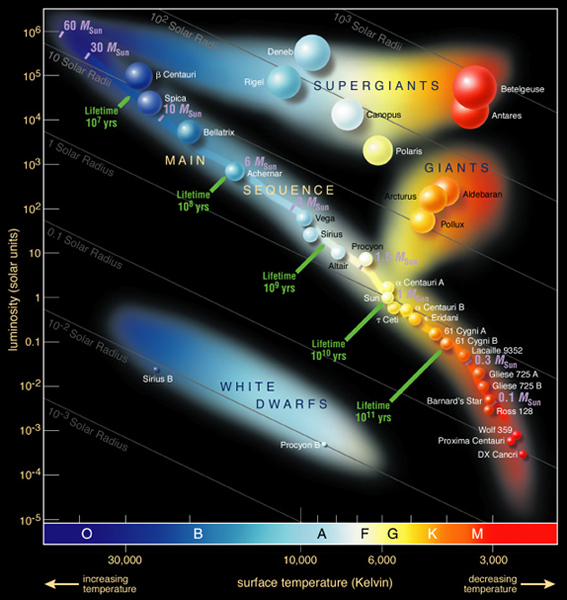
\includegraphics[scale=.30]{graphics/fig1}};
  \node[anchor=south west] at (0,-1)
  	{$\begin{aligned}
  	X &= (x_{1}, x_{2}, x_{3})\\
	C &= \{ c_1, c_2, c_3, c_4\} 
  	\end{aligned}$
  	};
 \end{tikzpicture}
\begin{textblock}{1}(0.505,.715)
  \footnotesize \texttt{Hertzsprung-Russell diagram}
 \end{textblock}
\clearpage


%slide3 ------------------------------------------------------------
\subsection{...and sometimes not.}

\begin{tikzpicture}[overlay]
  \node[anchor=south west] at (7.3,0.85) {$C = \{ ?\}$};
  \node[anchor=south west] at (5,-3.5) {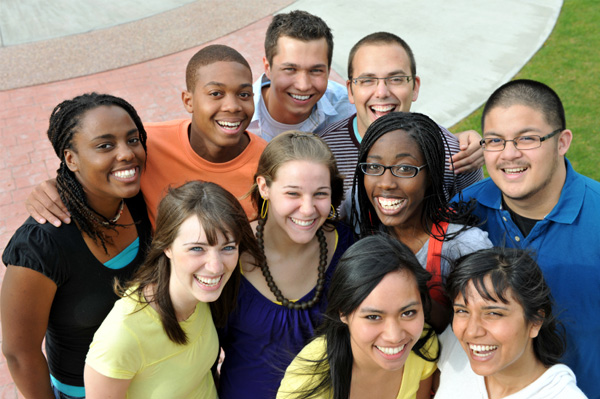
\includegraphics[scale=.30]{graphics/fig2}};
  \node[anchor=south west] at (1.3,-0.75) {$X = (?)$};
  \node[anchor=south west] at (0,-3.5) {
\includegraphics[scale=.10]{graphics/fig3}};
  
 \end{tikzpicture}
\clearpage


%slide4 ------------------------------------------------------------
\subsection{United Way's \textit{Breaking the Cycle of Childhood Poverty} campaign wants to:}
\begin{enumerate}
	\item Identify combinations of programs and services that can lead to predictable outcomes of success.
	\item Provide partner organizations with tools for in-house efficacy assessment of social service provisioning.
\end{enumerate}

\clearpage


%slide5 ------------------------------------------------------------
\subsection{Recommended:}
 \begin{enumerate}
  \item Write a proposal for a pilot project.
\end{enumerate}
\vspace{-7 mm}
\begin{myindentpar}{2 em}
\scriptsize  {... a pilot project for the development of machine learning tools ... \\
... for use by social service organizations ...\\
... use supervised learning algorithms called Naive Bayes classifiers ...}
\end{myindentpar}

\begin{tikzpicture}[overlay]
  \node[anchor=south west] at (2,-5.30) {
\includegraphics[width=0.60\textwidth, page=1]{graphics/project_proposal_20160516.pdf}}; 
 \end{tikzpicture}

\clearpage



%slide6 ------------------------------------------------------------
\begin{enumerate}[resume]
	\item Write a project plan document.
\end{enumerate}
\vspace{-7 mm}
\begin{myindentpar}{1em}
\scriptsize {... what is to be done, how it will be done ... \\
... who will be involved, who will have access to the results ...\\
... ethical safeguards, transparency guarantees, and legal frameworks ... \\
... for the entire project life cycle ...}
\end{myindentpar}

\begin{tikzpicture}[overlay]
  \node[anchor=south west] at (7.45,-1.65) {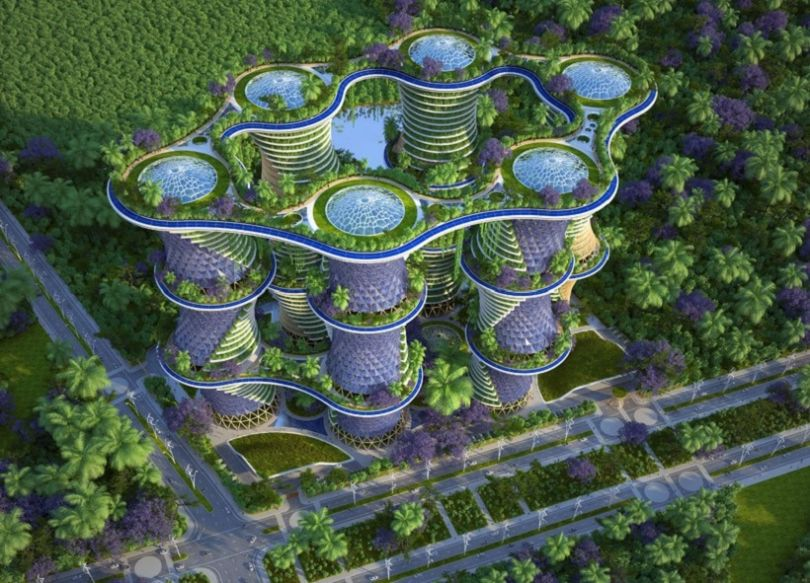
\includegraphics[scale=.20]{graphics/fig4}};
  \node[anchor=south west] at (2,-5.15) {
\includegraphics[width=0.43\textwidth, page=1]{graphics/project_plan_20160516.pdf}}; 
 \end{tikzpicture}

\clearpage


%slide7 ------------------------------------------------------------
 \begin{enumerate}[resume]
  \item Build and evaluate a set of Multinomial Naive Bayes classifiers.
\end{enumerate}
\vspace{-7 mm}
\begin{myindentpar}{1em}
\scriptsize {
...open source...\\
...readily available software...\\
...use Python-based, \enquote {MultinomialNB} from scikits-learn...}
\end{myindentpar}

\begin{tikzpicture}[overlay]
  \node[anchor=south west] at (4,-1.5) {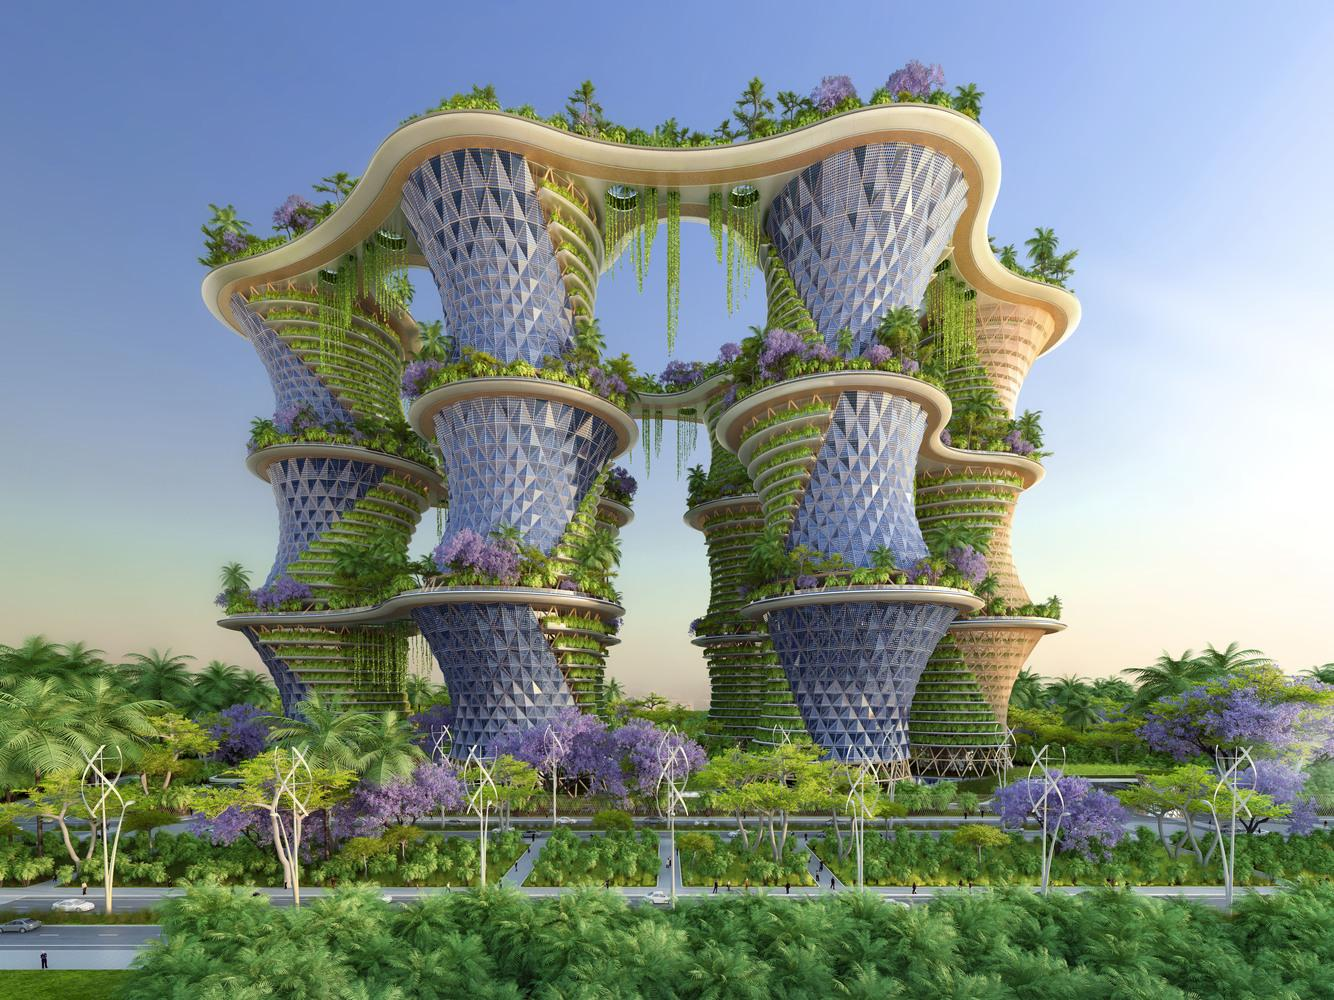
\includegraphics[scale=.30]{graphics/fig5}}; 
 \end{tikzpicture}

\clearpage


%slide8 ------------------------------------------------------------
\subsection{Naive Bayes Classifiers}
Naive Bayes classifiers are supervised learning algorithms that apply Bayes' theorem with the \enquote{naive} assumption of independence between every pair of features. \\
\\
Letting $C_k$ stand for the class variable with $k$ states and $\mathbf{x} = (x_1, \dots, x_n)$ stand for the features (data), then the Naive Bayes assumption is,
\begin{equation*}
p(x_i \vert x_{i+1}, \dots ,x_{n}, C_k ) = p(x_i \vert C_k)\
\end{equation*}

\clearpage


%slide9 ------------------------------------------------------------

and a Naive Bayes classifier gives,
\begin{align*}
p(C_k \vert \mathbf{x}) &= \frac{p(C_k) \ p(\mathbf{x} \vert C_k)}{p(\mathbf{x})}\\
P(C_k \mid x_1, \dots, x_n) &= \frac{P(C_k) P(x_1, \dots x_n \mid C_k)}{P(x_1, \dots, x_n)}\\
P(C_k \mid x_1, \dots, x_n) &= \frac{P(C_k) \prod_{i=1}^{n} P(x_i \mid C_k)}{P(x_1, \dots, x_n)}\\
P(C_k \mid x_1, \dots, x_n) &\propto P(C_k) \prod_{i=1}^{n} P(x_i \mid C_k)
\end{align*}

\clearpage


%slide10 ------------------------------------------------------------

Class assignment is then taken as,
\begin{equation*}
\hat{C_k} = \arg\max_{C_k} \ [ P(C_k) \prod_{i=1}^{n} P(x_i \mid C_k)]
\end{equation*}
(i.e., the class with the highest probability given the data)

\clearpage

%slide11 ------------------------------------------------------------
\subsection{The Trial Run}
Run MultinomialNB on Alpaydin's \enquote{OptDigits} database for the optical recognition of handwritten digits. Available from the UC Irvine Machine Learning Repository.
\vspace{-2 mm}
\begin{itemize}
	\item Training set has 3823 cases
	\item Test set has 1797 cases
	\item Each case has a feature vector with
	\begin{itemize}
		\item 63 measured values ranging from 0-16 (whole digits)
		\item a single class attribute corresponding to the natural number set, $N = \{0,1, 2,...,9\}$
	\end{itemize} 
\end{itemize}


\clearpage

%slide12 ------------------------------------------------------------
\subsection{The Data}
\verb!tr_d! = (3823 x 64) (\verb!n_cases, n_features!)\\
\verb!te_d! = (1787 x 64) (\verb!n_cases, n_features!)\\
\\
Head of \verb!tr_d!:
\vspace{-7 mm}
\footnotesize 
\begin{verbatim}
0,1,6,15,12,1,0,0,0,7,16,6,6,10,0,0,0,8,16,2,...,14,7,1,0,0,0
0,0,10,16,6,0,0,0,0,7,16,8,16,5,0,0,0,11,16,...,16,15,3,0,0,0
0,0,8,15,16,13,0,0,0,1,11,9,11,16,1,0,0,0,0,...,14,0,0,0,0,7
0,0,0,3,11,16,0,0,0,0,5,16,11,13,7,0,0,3,15,...,1,15,2,0,0,4
0,0,5,14,4,0,0,0,0,0,13,8,0,0,0,0,0,3,14,4,...,12,14,7,0,0,6
\end{verbatim}

\clearpage



%slide13 ------------------------------------------------------------

\begin{tikzpicture}[overlay]
  \node[anchor=south west] at (0,-5.5) {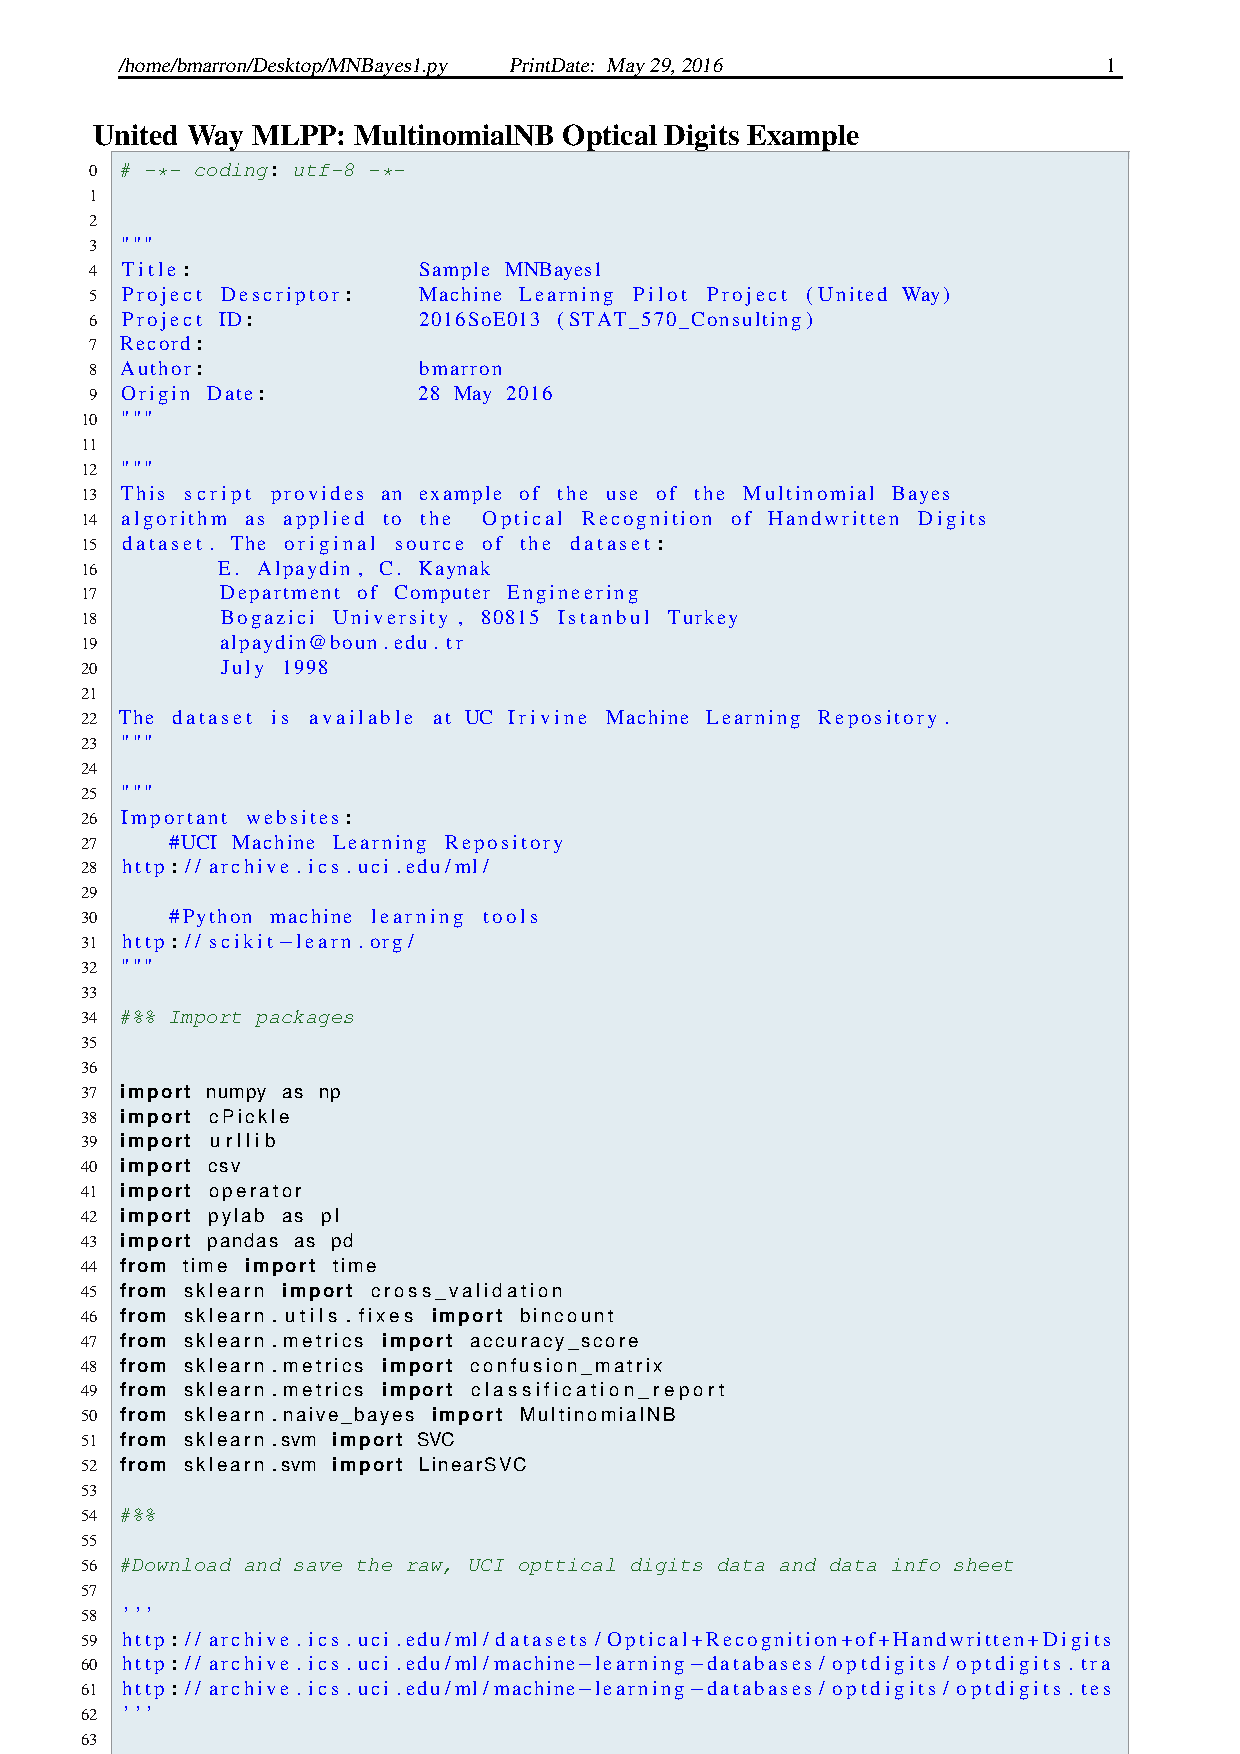
\includegraphics[width=0.45\textwidth, page=1]{graphics/MNBayes1.pdf}};
  \node[anchor=south west] at (5,-5.5) {\includegraphics[width=0.45\textwidth, page=2]{graphics/MNBayes1.pdf}};
  
   \end{tikzpicture}

\clearpage


%slide14 ------------------------------------------------------------
\subsection{The Results}
\scriptsize \begin{verbatim}
Testbenching a MultinomialNB classifier...
MultinomialNB(alpha=0.03, class_prior=None, fit_prior=True)
done in 0.016397s
Predicting the outcomes of the testing set
done in 0.006701s
\end{verbatim}

\begin{textblock}{1}(0.05,.50)
  \scriptsize  \texttt{Accuracy: 0.89} \\
  $ \left(\ddfrac{TP+TN}{\Sigma Total Population} \right)$
  \end{textblock}
  
 \begin{textblock}{1}(0.35,.55)
  \scriptsize  \texttt{Recall: 0.73-0.98} \\
  $\left(\ddfrac{TP}{(TP + FN)} \right)$
  \end{textblock}
  
  \begin{textblock}{1}(0.65,.60)
  \scriptsize  \texttt{Precision:0.76-0.99} \\
  $\left(\ddfrac{TP}{(TP + FP)} \right)$
 \end{textblock}

\clearpage


%slide15 ------------------------------------------------------------
\begin{textblock}{1}(0.05,.15)
  \scriptsize \texttt{Confusion matrix:}
 \end{textblock}
 
\begin{table}
\resizebox{.5\columnwidth}{!}{
\begin{tabular}{lrrrrrrrrrr}
\toprule
{} &    0 &    1 &    2 &    3 &    4 &    5 &    6 &    7 &    8 &    9 \\
\midrule
0 &  174 &    0 &    0 &    0 &    4 &    0 &    0 &    0 &    0 &    0 \\
1 &    0 &  132 &   19 &    0 &    0 &    1 &    6 &    0 &    9 &   15 \\
2 &    0 &    7 &  156 &    0 &    0 &    0 &    0 &    1 &   11 &    2 \\
3 &    1 &    0 &    2 &  154 &    0 &    2 &    0 &    6 &    9 &    9 \\
4 &    0 &    1 &    0 &    0 &  173 &    0 &    0 &    3 &    3 &    1 \\
5 &    0 &    0 &    0 &    0 &    1 &  165 &    1 &    0 &    2 &   13 \\
6 &    0 &    4 &    0 &    0 &    4 &    1 &  172 &    0 &    0 &    0 \\
7 &    0 &    1 &    0 &    0 &    1 &    0 &    0 &  173 &    3 &    1 \\
8 &    0 &   21 &    1 &    0 &    1 &    0 &    1 &    1 &  140 &    9 \\
9 &    0 &    1 &    0 &    6 &    4 &    1 &    0 &    1 &    7 &  160 \\
\bottomrule
\end{tabular}
}
\end{table}


\begin{tikzpicture}[overlay]
  \node[anchor=south west] at (6,-0.5) {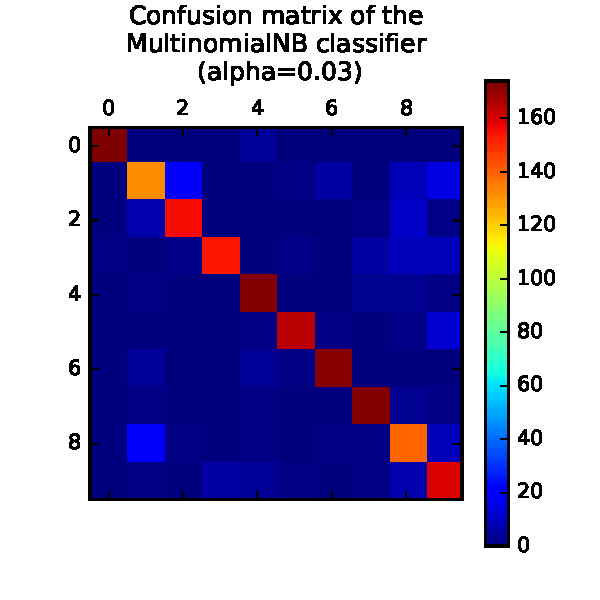
\includegraphics[width=0.45\textwidth, page=1]{graphics/MNBayes1_CM.pdf}};
   \end{tikzpicture}


\clearpage



%slide16 ------------------------------------------------------------
\subsection{Next Steps}
\begin{enumerate}
	\item Finalize the Machine Learning Pilot Project proposal document.
	\item Finalize the Project Plan document.
	\item Obtain a test dataset from Metropolitan Family Services.
	\item Run a Multinomial NB classifier.
	\item Evaluate and share results.
	\item Move to Phase II.
\end{enumerate}
\clearpage


%slide ------------------------------------------------------------
\begin{center}
\Large \textbf{Thanks!}
\end{center}
\clearpage


%slide ------------------------------------------------------------

\clearpage


%slide ------------------------------------------------------------
\subsection{Scientific Inference: From reality to models and back again}

\begin{tikzpicture}[overlay]
  \node[anchor=south west] at (0,-2.0) {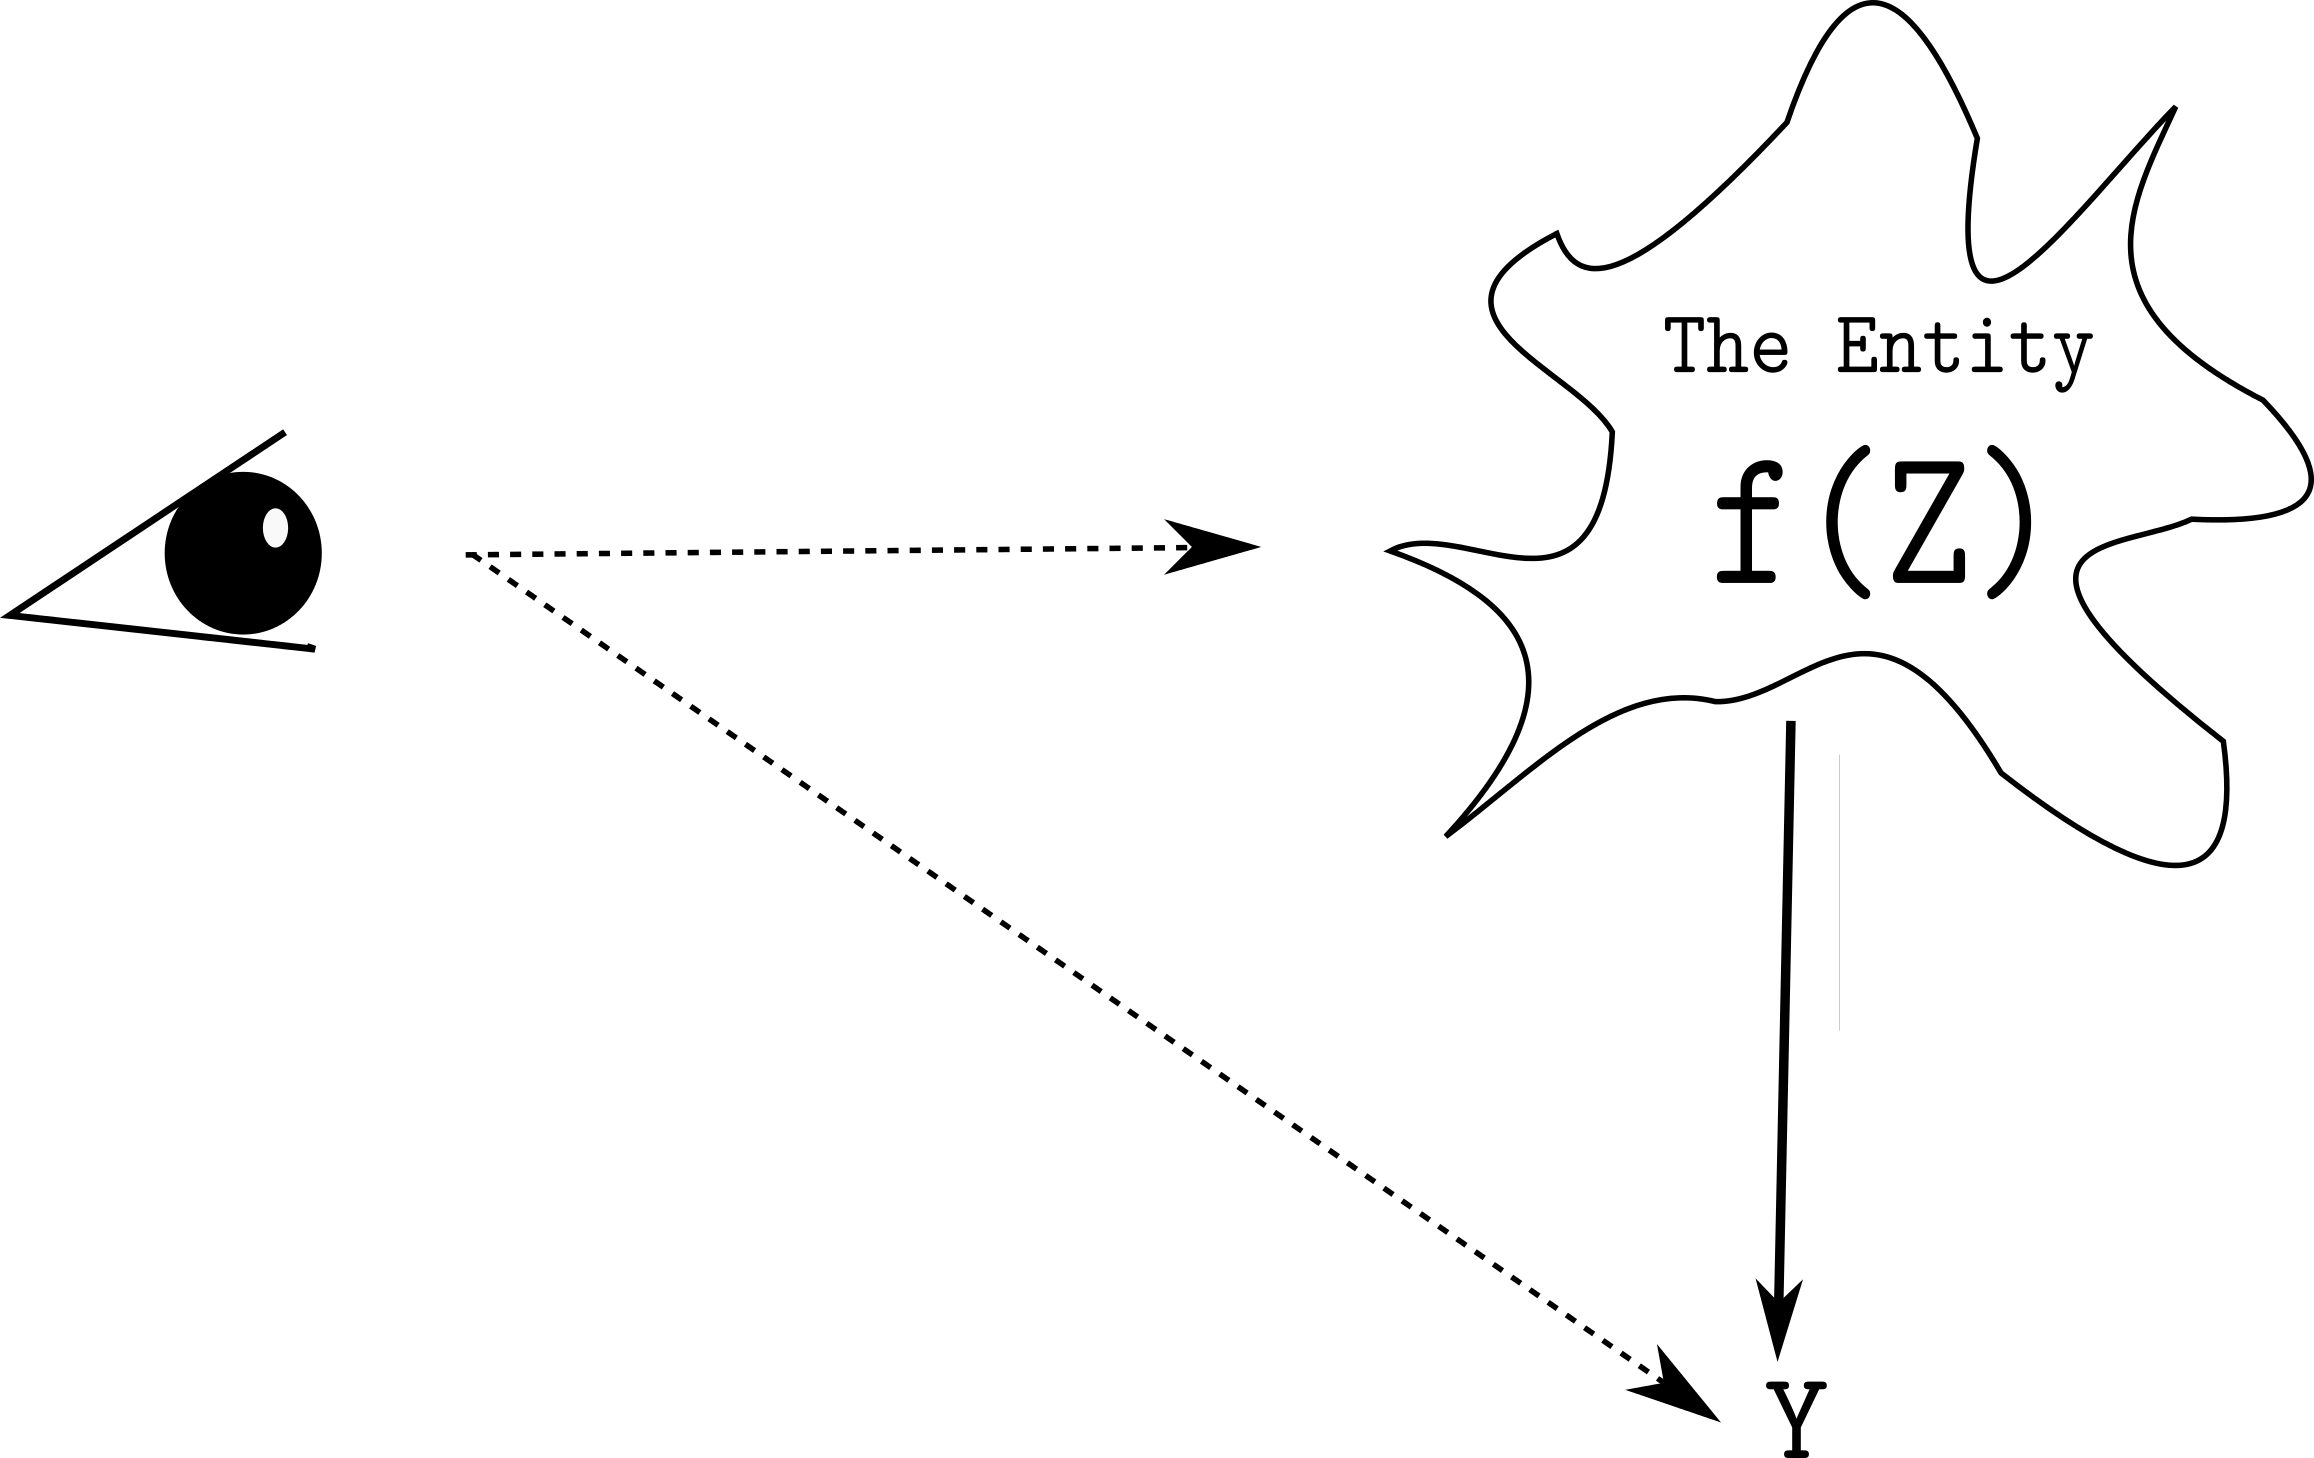
\includegraphics[scale=.35]{graphics/drawing1}}; 
 \end{tikzpicture}
 
 
 \begin{textblock}{1}(0.40,.25)
  \scriptsize {
  \begin{itemize}
  	\item We observe an entity in Nature that we suspect \\
  	generates non-random patterns of information
  	\item Our states of knowledge about the causal relationships \\
  	and processes, $f(\cdot )$, that are operating as well as about \\
  	the inputs,	$Z$, are limited; often severely	
  	\item We assume that some observable outcome, $Y$, is \\
  	\underline{causally} related to the entity as $f(Z) \Longrightarrow \{Y\}$  	
  \end{itemize}
  }
 \end{textblock}
 
 
\clearpage


%slide ------------------------------------------------------------
\subsection{Scientific inference: From reality to models and back again}

\begin{tikzpicture}[overlay]
  \node[anchor=south west] at (0,-2.0) {
\includegraphics[scale=.35]{graphics/drawing2}}; 
 \end{tikzpicture}
 
 \begin{textblock}{1}(0.40,.25)
  \scriptsize {
  \begin{itemize}
  	\item We assume that some observable and measurable \\
  	attributes (data), $\{X1, X2\}$ are \underline{logically} related \\
  	 to the entity's internal processes as, $\{X1, X2\} | f(Z) $ 
  	\item Lacking full knowledge of the entity's processes, we use \\
  	a probability model and consider $X1, X2, Y$ as random \\
  	variables with a joint probability distribution function
  	\item Lacking complete datasets, we accept sampled datasets
  	\item We make inductive inferences from the sampled datasets \\
  	back to	$f(Z)$ by assuming sampling distributions, \\
  	evaluating our prior knowledge, and using the (weaker) \\
  	syllogisms of plausible reasoning coupled with probability \\
  	theory
  \end{itemize}
  }
 \end{textblock}
 
 
 
\clearpage



%slide ------------------------------------------------------------

\clearpage


%slide ------------------------------------------------------------

\clearpage


%slide ------------------------------------------------------------

\clearpage






\end{document}
